\documentclass[12pt]{article}

%==============Packages & Commands==============
\usepackage{graphicx}
\usepackage{fancyvrb}
\usepackage{tikz}
%%%<
\usepackage{verbatim}
%\usepackage[active,tightpage]{preview}
%\PreviewEnvironment{tikzpicture}
%\setlength\PreviewBorder{5pt}%

\usepackage{geometry}                		% See geometry.pdf to learn the layout options. There are lots.
\geometry{a4paper}                   		% ... or a4paper or a5paper or ...
%\geometry{landscape}                		% Activat\usetikzlibrary{arrows}e for for rotated page geometry
%\usepackage[parfill]{parskip}    		% Activate to begin paragraphs with an empty line rather than an indent
\usepackage{graphicx}				% Use pdf, png, jpg, or eps§ with pdflatex; use eps in DVI mode
								% TeX will automatically convert eps --> pdf in pdflatex
\usepackage{amssymb}

\usepackage[ruled,vlined]{algorithm2e}
\usetikzlibrary{arrows}
\usepackage{alltt}
\usepackage[T1]{fontenc}
\usepackage[utf8]{inputenc}
\usepackage{indentfirst}
\usepackage[longnamesfirst]{natbib} % For references
\bibpunct{(}{)}{;}{a}{}{,} % Reference punctuation
\usepackage{changepage}
\usepackage{setspace}
\usepackage{booktabs} % For tables
\usepackage{rotating} % For sideways tables/figures
\usepackage{amsmath}
\usepackage{multirow}
\usepackage{color}
\usepackage{dcolumn}
\usepackage{comment}
%\usepackage{fullwidth}
\newcolumntype{d}[1]{D{.}{\cdot}{#1}}
\newcolumntype{.}{D{.}{.}{-1}}
\newcolumntype{3}{D{.}{.}{3}}
\newcolumntype{4}{D{.}{.}{4}}
\newcolumntype{5}{D{.}{.}{5}}
\usepackage{float}
\usepackage[hyphens]{url}
%\usepackage[margin = 1.25in]{geometry}
%\usepackage[nolists,figuresfirst]{endfloat} % Figures and tables at the end
\usepackage{subfig}
\captionsetup[subfloat]{position = top, font = normalsize} % For sub-figure captions
\usepackage{fancyhdr}
%\makeatletter
%\def\url@leostyle{%
%  \@ifundefined{selectfont}{\def\UrlFont{\sf}}{\def\UrlFont{\small\ttfamily}}}
%\makeatother
%% Now actually use the newly defined style.
\urlstyle{same}
\usepackage{times}
% \usepackage{mathptmx}
%\usepackage[colorlinks = true,
%						bookmarksopen = true,
%						pagebackref = true,
%						linkcolor = black,
%						citecolor = black,
% 					urlcolor = black]{hyperref}
%\usepackage[all]{hypcap}
%\urlstyle{same}
\newcommand{\fnote}[1]{\footnote{\normalsize{#1}}} % 12 pt, double spaced footnotes
\def\citeapos#1{\citeauthor{#1}'s (\citeyear{#1})}
\def\citeaposs#1{\citeauthor{#1}' (\citeyear{#1})}
\newcommand{\bm}[1]{\boldsymbol{#1}} %makes bold math symbols easier
\newcommand{\R}{\textsf{R}\space} %R in textsf font
\newcommand{\netinf}{\texttt{NetInf}\space} %R in textsf font
\newcommand{\iid}{i.i.d} %shorthand for iid
\newcommand{\cites}{{\bf \textcolor{red}{CITES}}} %shorthand for iid
%\usepackage[compact]{titlesec}
%\titlespacing{\section}{0pt}{*0}{*0}
%\titlespacing{\subsection}{0pt}{*0}{*0}
%\titlespacing{\subsubsection}{0pt}{*0}{*0}
%\setlength{\parskip}{0pt}
%\setlength{\parsep}{0pt}
%\setlength{\bibsep}{2pt}
%\renewcommand{\headrulewidth}{0pt}

%\renewcommand{\figureplace}{ % This places [Insert Table X here] and [Insert Figure Y here] in the text
%\begin{center}
%[Insert \figurename~\thepostfig\ here]
%\end{center}}
%\renewcommand{\tableplace}{%
%\begin{center}
%[Insert \tablename~\theposttbl\ here]
%\end{center}}

\newcommand\independent{\protect\mathpalette{\protect\independenT}{\perp}}
\def\independenT#1#2{\mathrel{\rlap{$#1#2$}\mkern2mu{#1#2}}}
\newcommand{\N}{\mathcal{N}}
\newcommand{\Y}{\bm{\mathcal{Y}}}
\newcommand{\bZ}{\bm{Z}}

\usepackage[colorlinks = TRUE, urlcolor = black, linkcolor = black, citecolor = black, pdfstartview = FitV]{hyperref}


%============Article Title, Authors==================
\title{\vspace{-2cm} Inference on the Effects of Observed Features 
\\ in Latent Space Models for Networks } 


\author{ Zachary Jones \and Matthew Denny \and Bruce Desmarais \and Hanna Wallach} \date{\today}



%===================Startup=======================
\begin{document}
\maketitle



%=============Abstract & Keywords==================

\begin{abstract}

\noindent The latent space model (LSM) for network data is a popular model that combine a generalized linear model with a latent spatial embedding of the network to model ties. It has been used to decrease error in the estimation of and inference regarding the effect of observed covariates. In applications of the LSM, it is assumed that the latent spatial embedding can control for unmeasured confounders that have an effect on the value of edges in a network. We investigate the latent space model's performance on this task via a Monte Carlo simulation wherein we show that in the presence of an unmeasured covariate which can be appropriately modeled using a latent space, estimation and inferential error does decrease. However, when no such unmeasured covariate is present, a generalized linear model substantially outperforms the latent space model. The LSM is often biased downwards by nearly half the magnitude of the coefficient of the observed covariate. This pattern is repeated with generalization error and with type 1 and type 2 error rates. We investigate solutions to this issue and conclude with recommendations as to the appropriate use of the latent space model for observational studies.

\end{abstract}
\thispagestyle{empty}
% \doublespacing
% Description of the possible challenges
\section{Introduction}

\subsection{Problem}

Latent variable inference, generally conceived, presents the possibility of representing unmeasured data in statistical models. The latent space model (LSM) \cite{hoff2002latent} for network data is regularly used to estimate the effect of covariates in the presence of latent network structure. However, it is unclear that the introduction of a latent space decreases the expected error for the parameter(s) of interest when aspects of the network structure (e.g., homophily) that are unmeasured are correlated with measured covariates. There are two reasons that using the LSM may lead to increased error. First, the latent configurations inferred may result in a representation of the network wherein a node's position in the latent space is spurriously correlated with the observed covariates, leading to reduced efficiency due to multicollinearity. Second, if the unobserved (i.e., latent) network structure is truly correlated with the observed covariates, the unobserved structure that can be correlated with the observed variable may be attributed to the observed variable, while the latent space parameters are used to model other sources of variation.

In what follows we identify the conditions under which using the LSM reduces the estimation and inferential error with respect to the effects of observed covariates. We compare the performance of LSM to the generalized linear model (GLM) as a baseline. We develop a simulation design in which we control the degree of collinearity between omitted network structure and observed covariates. We investigate whether the prior can be tuned to avoid efficiency losses in using the LSM. We conclude with recommendations regarding the ideal use of the LSM.

\section{Background}

\subsection{Applications and Development of the Latent Space Model}

The LSM has seen use in a variety of fields in which network data is common, particularly the social sciences. This appeal appears to have been driven primarily by the LSM's usefulness in modeling transitivity and homophily which appear to be ubiquitous in many (social) networks. In political science the LSM and variations on the form developed in \cite{hoff2002latent} have been used to estimate the effect of democracy on the probability of a militarized interstate dispute \citep{ward2007disputes}, the amount of portfolio investment between states \citep{cao2013democracies}, and the effect of multimember districts on the probability of collaboration between state legislators in the United States \citep{kirkland2012multimember}. Variations of the LSM developed for networks measured over time have been applied to the study of international trade, wherein the effects of various features of trading partners are estimated \citep{ward2013gravity}. In ecology the LSM has been used to study the sociality of elephants \citep{vance2009social} and orcas \citep{fearnbach2014spatial}, to discover ecological communities \citep{fletcher2011social, fletcher2013network}, and to study food webs \citep{chiu2011unifying}. In epidemeology the LSM has been used to identify clusters of infected persons for later isolation \citep{zhang2015cluster} and to study patterns of interaction amongst physicians \citep{paul2014results}. In marketing and business research the LSM has been used to study inter-group trust \citep{dass2011impact}, optimal bundling and pricing of goods and brands for retailers \citep{dass2012assessing}. In neuroscience the LSM has been proposed as a method for modelling fMRI data \citep{simpson2013analyzing}.

% need to add marketing stuff and probably should look again for applications
% also need to read and fit in the newer ward student stuff

Although the latent space model is arguably most useful as an exploratory or predictive model \citep{hoff2002latent, shmueli2010explain} it has been applied in some cases in a manner that suggests that users of the model assume that the latent space parameters reduce estimation and/or inferential error with respect to the effects of measured explanatory variables. Though it is not the case that all of the aforementioned articles explicitly or implicitly make such a claim (not all of the above applications of the LSM even include covariates), if the LSM does reduce inferential/estimation error under certain conditions, the LSM might find wider use due to the pervasiveness of network data where there remains unmeasured structure which either confounds relationships between measured covariates and edges, in which case the LSM might be applied to reuduce bias, or in which unmeasured structure is related to the strength/presence of edges and can be useful in decreasing estimator variance. Additionally, the predictive performance of the LSM has only seen limited evaluation \citep{hoff2002latent}, despite having been used for model selection \citep{ward2013gravity, fletcher2011social, fletcher2013network, chiu2011unifying}. Hence, finding the condtions under which the LSM reduces prediction error also may affect future use of the LSM.

The LSM has also seen a substantial amount of subsequent development and extension. The latent space has been represented as a $k$-dimensional Euclildean space and by latent factors \citep{hoff2002latent, hoff2009multiplicative}. Additional structure has been introduced by adding random effects, which, for example, may involve sender or receiver specific effects for directed networks which capture differential activity rates amongst nodes \citep{hoff2003random}. Within this framework \cite{westveld2011mixed} models dynamic network data by treating the latent space as a stochastic process. \cite{handcock2007model} enable the LSM to model clustering that is not representable as homophily (i.e., stochastic equivalence) by combining the LSM with latent cluster models. \cite{hoff2008modeling} shows that the LSM and latent cluster models are special cases of an ``eigenmodel.'' That is, an eigendecomposition of a symmetric sociomatrix can be used to represent both latent space and cluster models, 
but not vice-versa.

\subsection{Collinearity in Generalized Linear Models}

\citep{mackinnon1989collinearity} and \citep{weissfeld1991multicollinearity} investigate multicollinearity in generalized linear models and propose diagnostic criteria. Collinearity of the covariates causes the observed information matrix to be ill-conditioned, which produces nmerical instability in the iterative esimation of $\hat{\mathbf{\beta}}$. \citep{weissfeld1991multicollinearity}, extending the work of \citep{davis1986example}, propose the use of the condition index and the variance decomposition proportion of each condition index, to diagnose the presence and degree of multicollinearity in generalized linear models. The observed information matrix at the maximum likelihood estimate, $\mathcal{I}(\hat{\mathbf{\beta}})$ is scaled to have unit length and singular value decomposition is applied. The resulting right singular values are the eigenvectors and the associated singular values are the square root of the eigenvalues of the scaled observed information matrix since it is real Hermitian. The condition index is the ratio of the largest eigenvalue to each of the eigenvalues, and is at least 1. The square root of the condition number gives the potential magnification of the numerical error in inverting the observed information matrix. Hence our expectation is that as collinearity increases the variance of estimators of the effect of observed covariates will increase regardless of whether this is ommitted confounding structure in the data.

\section{Research Design}

\subsection{Priors for the Latent Space Model}

\subsubsection{Current Implementations}

What priors are currently used and why? \cite{hoff2002latent} Propose the use of diffuse independent normal priors for the latent positions and regression parameters. The also recognize the fact that isolates' positions are weakly identified in the LSM, and in one application they actually just exclude the isolate.\footnote{Excluding isolates seems fine if the inferential purpose is to estimate positions in the latent space. However, such deletion would introduce bias in estimating covariate effects.} \cite{hoff2002latent} experiment with the use of an exponential prior for the intercept, which they argue sets a lower bound on the probability of a tie between nodes. Of course, the latent space positions could simply drift further apart in order to compensate for the high intercept. The following paragraph on priors appears on page 1097.

\begin{quote}
We have not discussed in detail the choice of a prior distribution for latent positions in this article. Although simple, the diffuse independent normal priors presented in the examples may not accurately represent prior beliefs about the structure of social networks. More appropriate might be clustered point processes or mixtures of normals with an unknown number of components. Such priors could allow one to incorporate prior information on tendencies for clustering, without specifying cluster membership. This would add another level of hierarchy to the analysis, although the resulting model would be more flexible and perhaps more accurately represent any tendencies of populations to form segregating groups.
\end{quote}

\citep{Krivitsky2009} implement a hierarchical model in which each node's latent space position is drawn from a mixture of $G$ normals. The covariate priors are single Gaussians.

\subsubsection{Alternatives to consider}

Would regularization/sparsity priors help with identifying the covariate effects? \cite{mitchell1988} propose a class of ``spike and slab'' prior as a class of priors for the coefficients in linear regression.  These priors are well-suited to the problem of variable selection for linear regression. The prior is formed as a mixture between a diffuse uniform prior and a point mass at zero. Such a prior would not be appropriate for latent space coordinates since weakly identified coordinates of isolates or separate components would likely exhibit strange behavior at the boundary of the diffuse uniform. We might consider instead mixing, e.g., a point mass at zero with a distribution such as the Cauchy, which is fairly flat in the tails, but is defined on the entire real line and still exhibits a surface that descends from the center of the distribution. This prior structure would build a preference into the model for using the observed covariates, rather than the latent coordinate parameters, to explain tie formation.

What priors could be used to avoid collinearity between observed covariates and latent space? Look to Bayesian Latent Trait models and specifically differential item functioning (DIF) in the IRT literature.

Should priors be calibrated against observed covariates? Using informative priors assures that the latent space coordinates are weakly identified, meaning that at some distance from the origin the increase in the likelihood from moving isolates away from the other nodes, or components away from each other, is offset by decreases in the prior from moving coordinates away from the origin. However, we may also use the priors to penalize the model for inferring latent coordinates that result in distances that are comparable in scale to the observed covariates. This would embed a tendency for the model to use the observed covariates, rather than the latent space, to model the outcome. Consider the following example of a one-dimensional spatial model with an additional dyadic covariate. 

$$ pr(y_{ij} = 1) = \text{logit}^{-1}(\beta_0 + \beta_1x_{ij} -  |z_i - z_j|).$$

If we assume that the $z$ are independent and distributed $N(0,\sigma^2)$, it is straightforward to derive the distribution of $ |z_i - z_j|$.\footnote{The assumption that $z \sim N(0,\sigma^2$) is consistent with $z$ being drawn from the prior that is conventionally used in the LSM.} Since it is a special case of a ``normal difference distribution'', we know that $z_i - z_j \sim N(0,2\sigma^2)$ \citep{devore2012}. The normality of $z_i - z_j$ implies that $|z_i - z_j|$ has a folded normal distribution \citep{leone1961}. Following from this result, we know that the variance of  $|z_i - z_j|$ is $$\sigma^2(2-4/\pi). $$ Let $\alpha^2$ be the empirical variance of $x$. Then the variance in the linear predictor is $\beta_1^2\alpha^2$. Given an estimate $\hat{\beta_1}$, we can set the variance of the latent space prior to approximately $\hat{\beta_1}^2\alpha^2/(2-4/\pi)$ in order to tune the prior to avoid replicating $x$ via the distances between latent coordinates. This result is limited in that it requires the assumption of normally distributed latent coordinates and applies only to a single latent dimension. However, it may provide a reasonable approximation in the case of non-normal coordinates and/or multiple dimensions. 

\cite{thirey2015} derive the distribution of Euclidean Distances between two $k$-dimensional points where each coordinate is drawn from a standard normal distribution.

\subsection{Tasks}
\begin{itemize}
\item Review multicollinearity issues in GLM (ZJ)
\item Describe how multicollinearity will manifest in LSM (ZJ)
\item Delve into LSM priors (BD)
\begin{itemize}
\item Scaling variance to observed covariates
\item Spike and slab
\item Covariance
\end{itemize}
\end{itemize}

\section{Analysis}

\subsection{simulation design}

To study how the LSM behaves in the situation in which we have some observed covariates as well as omitted network structure which can be represented using a Euclidean latent space. For simplicity we consider a unidimensional latent space. To generate an observed covariate which has a controllable collinearity with the latent network structure we follow a three-step process. First, we simulate $k$-dimensional positions for each node, drawing each from a normal distribution, and calculate dyadic distances $d$ between each pair of positions. Second, given a target covariance matrix ($\Sigma$) among the covariates and distances, $\langle X,d \rangle$, we derive the conditional mean vector and covariance, assuming that $X$ has a joint normal distribution given $d$ (see \cite[pp. 116--117]{eaton1983} for the conditional normal derivation). Third, we simulate $X$ as a multivariate normal random variable with the respective conditional means and covariance. Finally we standardize each $X$ to have 0 mean and unit variance. To generate the covariance matrix $\Sigma$ which controls the dependence between the omitted network structure and the observed covariate $X$ we utilize the C-vine method of \cite{lewandowski2009generating}. % fill in a basic description of the method here

We consider three exponential family distributions for the edges: Gaussian, Binomial, and Poisson. Additionally we control the number of nodes in the network $n = 25, 50, 100$, fix the dimension of the latent space $k$ at 1 for simplicity, and consider 5 values of the collinearity parameter $\eta$, equally spaced between $.75$ and $100$, where $.75$ corresponds to near perfect collinearity and $100$ to independence.

We standardize $X$ to have a variance of $1$ and a mean of $0$.

\begin{figure}
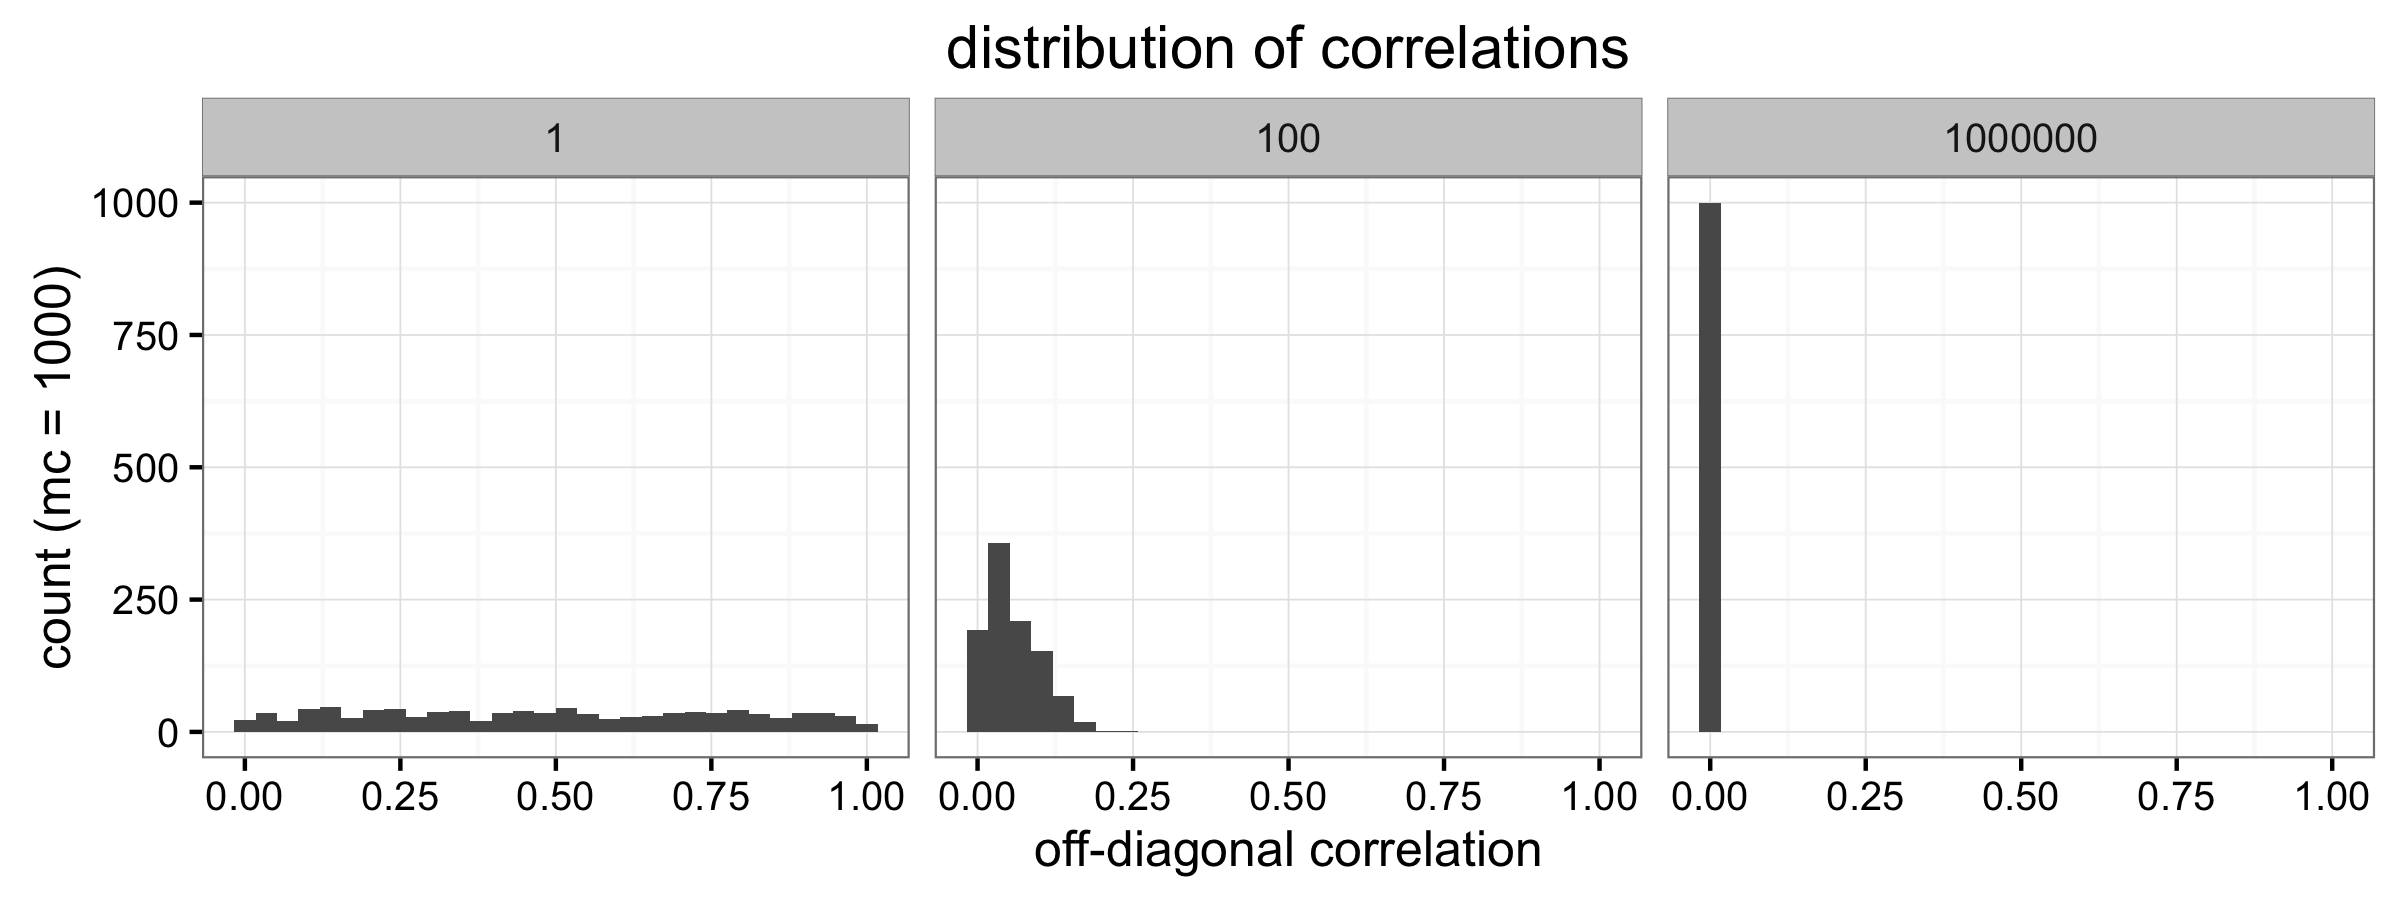
\includegraphics[width=\textwidth]{max_r_vine.png}
\caption{The distribution of the absolute value of the maximum off-diagonal correlation.}
\end{figure}

Each step in the simulation involves the estimation of a GLM, the LSM, and the LSM with a prior on the latent space which is scaled by $\hat{\beta_1}^2\alpha^2/(2-4/\pi)$, where $\alpha^2$ is the empirical variance of $X$. At each step in the simulation, the LSM is estimated using the canonical implementation in the \texttt{latentnet} package in \texttt{R}. An initial run of 10,000 burn in iterations, followed by 1,000,000 iterations of the sampler. Every 100th iteration is saved. Convergence in the log probability of the model is assessed using the Geweke diagnostic. If the convergence criteria is satisfied the simulation continues to the next set of arguments, otherwise the number of iterations is doubled. If the convergence criteria is still not satisfied, then the aforementioned step in the simulation is flagged for review. At each point in the simulation's parameter space, we execute 500 Monte Carlo iterations.

We first compute the MLE estimated by iteratively reweighted least squares in \texttt{R}. For the LSM we use the posterior mode. In the cases where edges are Binomial distributed, we scale the estiamtes using the reciprocal of the bias of $\beta_1$ when $X$ and $d$ are independent: $\frac{\sqrt{3.28 + \beta_2^2 \text{Var(d)}}}{\sqrt{3.29}}$, where $3.29$ is the variance of a standard logistic distribution \cite{mood2010logistic}.

To evaluate estimation error we compute the bias: the difference between the true coefficient $\beta_1$ and the estimate. Figure \ref{fig:estimation} shows the results. When a latent space is present (i.e., $\beta_2 = -1$) the LSM outperforms the GLM in terms of bias across the board. However, when latent network structure is not present ($\beta_2 = 0$) the LSM is sharply biased downwards, indicating that the latent space is representing variability in the edges that is attributable to the observed covariate $X$.

\begin{figure}
\includegraphics[width=\textwidth]{estimation.png}
\caption{The bias of estimates of the effect of the observed covariate $X$. The $x$-axis gives the value of the parameter $\eta$, which controls the degree of dependence between $X$ and ommitted covariate. Lower values of $\eta$ indicate higher levels of dependence between the observed and ommitted covariate. The $y$-axis gives a Monte Carlo estimate of the bias, and the grey ribbon gives a pointwise 95\% confidence interval for the Monte Carlo estimate. The number of nodes and the presence or absence of omitted network structure are indicated in the top panels, while the distributional family for the edges and the value of the coefficient for $X$, $\beta_1$ are indicated on the right panels. Each panel represents 3 values of $\eta$ with 500 Monte Carlo iterations executed at each point.
\label{fig:estimation}}
\end{figure}

We consider networks of varying size (i.e. number of nodes), density (i.e., the number/strength of edges between nodes), and collinearity structure between the ommitted distance between nodes and the measured covariates. For each point in this space we evaluate the mean square prediction error of the model on new data drawn from the same distribution (i.e., the generalization error), the bias of the estimated coefficients for the measured covariate, the type 2 error rate (i.e., the probability that the null hypothesis that each regression parameter is $0$ is incorrectly accepted), and the type 1 error rate, that is, the probability of rejecting the null hypothesis that the effect of the measured covariate is 0 when it is in fact 0. Inference regarding $\boldsymbol\beta$ is computed using the maximum a posteriori estimate (i.e., the mode of the posterior), and credible sets for $\boldsymbol\beta$ are defined by using the region of highest posterior density which covers $95\%$ of the marginal posterior distribution for each regression parameter.

\begin{figure}
\includegraphics[width=\textwidth]{inference.png}
\caption{Monte Carlo estimates of the Type-1 and Type-2 error regarding the effect of the observed covariate $X$ are shown on the $y-axis$. When the right gray panel indicates ``Type-1'' $\beta_1 = 0$ and the error rate shown in each panel in that row gives 1 minus the probability of a 95\% confidence region (for the LSM) or interval (for the GLM) including $0$, giving the probability that a true null hypothesis of $\beta_1 = 0$ is falsely rejected. When the right gray panel indicates ``Type-2'' then $\beta_1 = 1$ and the error rate shown in each panel in that row gives the probability of the probability/confidence intervals covering $0$, giving the probability of accepting a false null hypothesis. The $x$-axis gives the value of the parameter $\eta$, which controls the degree of dependence between $X$ and ommitted covariate. Lower values of $\eta$ indicate higher levels of dependence between the observed and ommitted covariate. The grey ribbon gives a pointwise 95\% confidence interval for the Monte Carlo estimate. The number of nodes and the presence or absence of omitted network structure are indicated in the top panels, while the distributional family for the edges and the value of the coefficient for $X$, $\beta_1$ are indicated on the right panels. Each panel represents 5 values of $\eta$ with 500 Monte Carlo iterations executed at each point. \label{fig:inference}}
\end{figure}

\begin{figure}
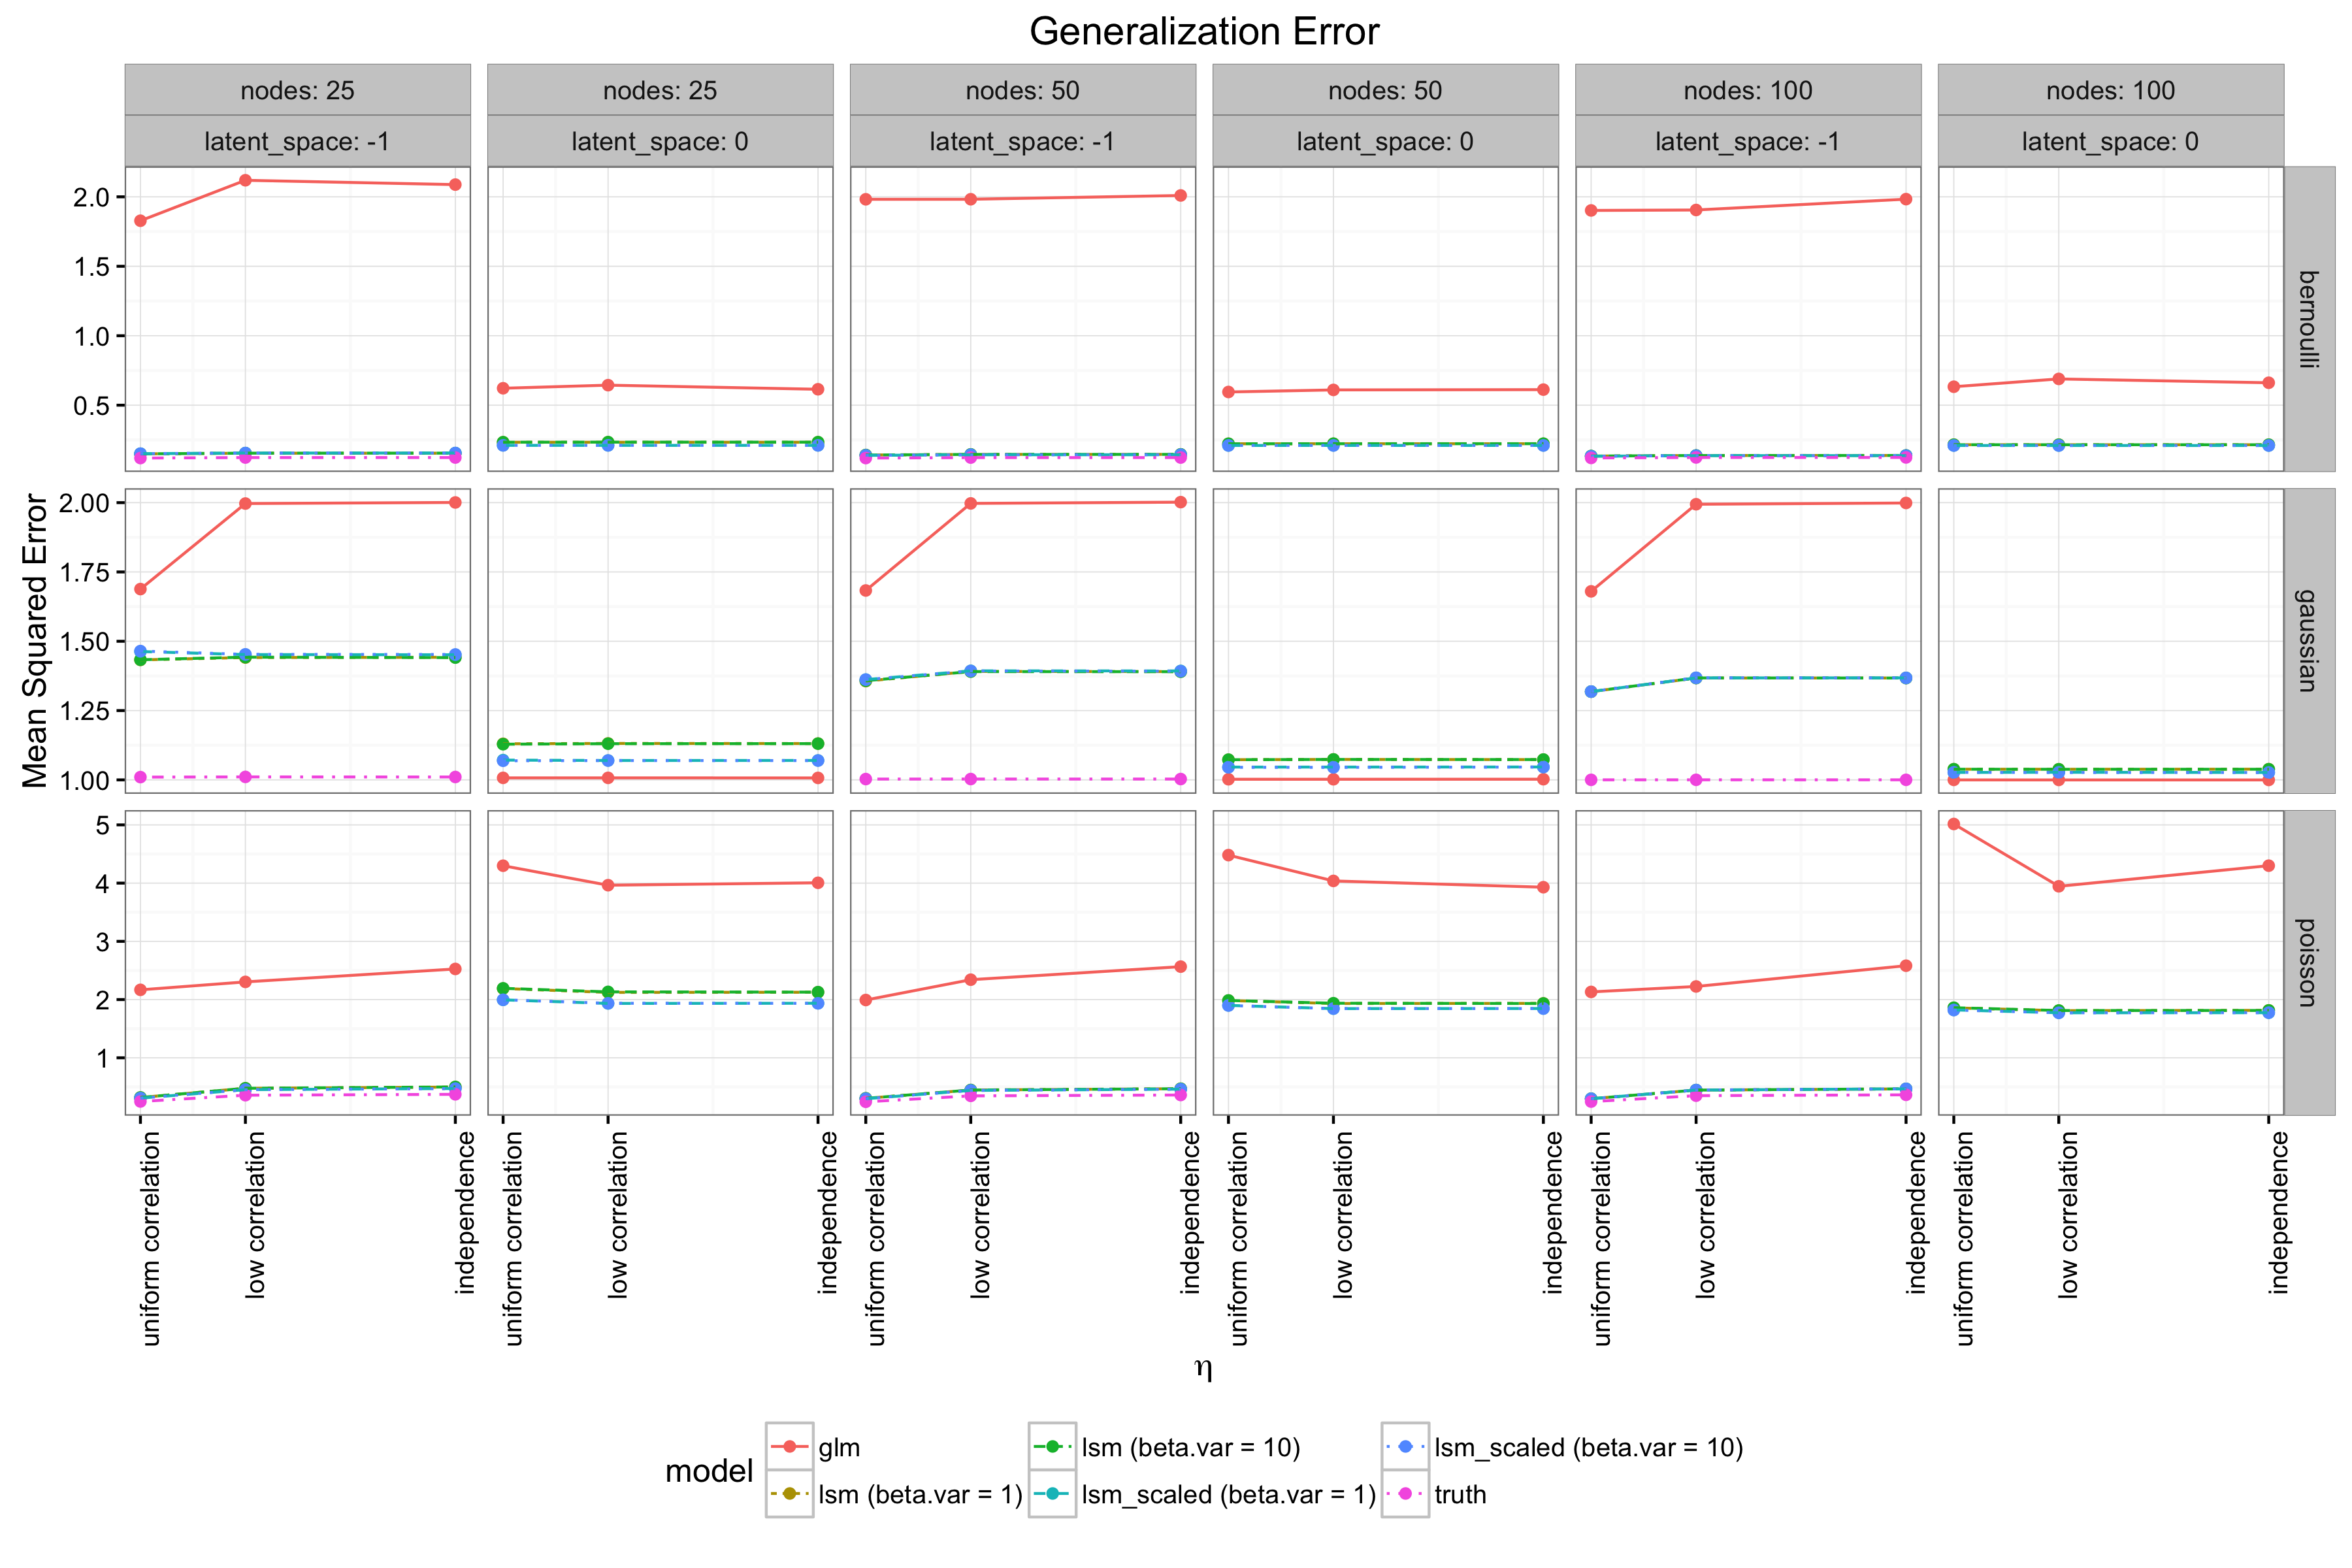
\includegraphics[width=\textwidth]{generalization.png}
\caption{The $x$-axis shows a Monte Carlo estimate of the mean square error for edge values drawn from the generative model using a model trained on independent data. The $x$-axis gives the value of the parameter $\eta$, which controls the degree of dependence between $X$ and ommitted covariate. Lower values of $\eta$ indicate higher levels of dependence between the observed and ommitted covariate. The grey ribbon gives a pointwise 95\% confidence interval for the Monte Carlo estimate. The number of nodes and the presence or absence of omitted network structure are indicated in the top panels, while the distributional family for the edges and the value of the coefficient for $X$, $\beta_1$ are indicated on the right panels. Each panel represents 5 values of $\eta$ with 500 Monte Carlo iterations executed at each point. \label{fig:generalization}}
\end{figure}

One of the primary difficulties in executing the above simulation design is the computational cost of estimating the LSM. We utilize the \texttt{BatchJobs} and \texttt{BatchExperiments} \R packages to construct and execute our computational experiments on a Torque cluster \cite{bischl2015batchjobs}.

\newpage

\bibliographystyle{apsr}
\bibliography{ref}

\end{document}